\chapter{Equivalence, Observation, and Refinement}
\label{ch:equivalence-refinement}

Two programs can produce the same answer and still disagree about memory,
conditions, traps, running time, or whether they return at all. They can agree
for one caller and fail for another. They can implement the same mathematical
operation while inhabiting machine states with no matching register names.
The word \emph{equivalent} becomes useful only after these choices are fixed.

This chapter turns agreement into a statement with visible parts. A
precondition selects inputs. Program semantics produces behavior. An
observation selects what the claim exposes. Equivalence compares programs in
one state space. Refinement relates programs whose states or permitted
behaviors differ. A counterexample supplies an allowed input and an inspectable
execution that breaks one required clause.

\begin{keyidea}[title={Equivalence is always relative to a contract}]
Name the initial states, termination policy, trap policy, observation, and
program semantics. If a surrounding context will use the replacement, name
what that context may read. Without those parts, ``same program'' is an
intuition rather than a theorem statement.
\end{keyidea}

\section{Why program agreement became a central problem}

Programmers have replaced instruction sequences for as long as they have
optimized code. A hand optimizer shortened an address calculation. A compiler
reordered operations or allocated another register. A \keyterm{linker}, the
tool that combines object files, relaxed a long
transfer into a shorter one. Each transformation carried an implicit promise:
the change would not alter what mattered to the rest of the program.

Modern systems make that promise at larger scale. Optimizing compilers perform
thousands of rewrites. Binary translators move code between instruction sets.
Cryptographic implementers replace clear scalar formulas with sequences chosen
for speed or side-channel discipline. Superoptimizers search for a least-cost
program within a declared language. Formal tools compare implementations with
specifications. All depend on a defensible meaning of agreement.

The strongest meaning is often unnecessarily strict. A scratch register may
differ after a closed function. Temporary condition bits may be dead. A source
machine may have no counterpart for a target machine's flags. The weakest
meaning is unsafe: comparing only the desired numeric result can hide a trap,
wrong return address, or caller-owned memory corruption. The task is to choose
the smallest observation that still protects every permitted use.

\begin{archive}[title={Optimization is a promise about the future}]
A replacement is not justified merely because two isolated executions look
alike. It is justified when every allowed future use receives the behavior the
contract promised. Context gives local equality its program-wide meaning.
\end{archive}

\section{Programs produce behaviors, not only final values}

Let \(P\) be a deterministic program and \(S\) an allowed initial state. Its
execution may reach a normally halted state, reach a trapped state with a
reason, or continue without a terminal state. Write
\[
  \mathit{Beh}(P,S)
\]
for that behavior. A finite bounded runner may also stop because its external
step budget is exhausted, but bound exhaustion is evidence about a prefix,
not a fourth architectural behavior.

For a terminating behavior, let \(\mathit{final}(P,S)\) denote the terminal
state. A normal-result observation \(A\) is applied only where its domain is
defined. A total behavior observation can instead map normal return, trap, and
divergence to distinct forms while applying \(A\) to a normal final state.

\begin{definition}[title={Termination-sensitive observed behavior}]
Fix an observation \(A\). The observed behavior \(B_A(P,S)\) reports one of:
normal return together with \(A\) of the final state; trap together with the
declared trap observation; or divergence. Two executions agree only when
these outer behavior classes agree and their exposed contents agree.
\end{definition}

Divergence is a mathematical property of an unbounded execution. A thousand-
step prefix does not establish it. Conversely, a termination argument may use
an invariant and decreasing measure without enumerating the entire trace.
Chapter 9's counted loop supplied exactly that form of reasoning.

Some claims intentionally use \keyterm{partial correctness}: if both programs
return normally, their results agree, but termination is handled elsewhere.
That statement can be valuable, yet it does not authorize replacing a
terminating program with a diverging one. The theorem and its use must retain
the weaker termination policy in the name or scope.

\begin{warning}[title={A result observation must not erase behavior class}]
If one execution returns \(r_0=7\) and another traps after previously writing
\(r_0=7\), projecting both states to \(r_0\) hides the difference. Compare
normal, trapped, and divergent behavior before comparing a result value.
\end{warning}

\subsection{When one input can have several behaviors}

The selected A0, RV64I, and x86-64 slices are deterministic: a legal running
state has at most one next architectural state. Larger models may admit several
behaviors from one input. A source language may leave evaluation order
unspecified. A concurrent machine may allow several event orders. An abstract
specification may intentionally permit several implementation choices.

Then \(\mathit{Beh}(P,S)\) is a set rather than one item. Agreement can mean
set equality, inclusion, or agreement on selected possibilities. A refinement
often requires every implementation behavior to be allowed by the
specification:
\[
  \mathit{Beh}(Q,T)\subseteq \mathit{Beh}(P,S)
\]
for related inputs. The implementation may resolve choices, but it may not add
an outcome forbidden by the specification.

Two common questions differ. A \keyterm{may} property asks whether at least one
allowed execution has an observation. A \keyterm{must} property asks whether
every allowed execution has it. Showing that two programs can both return 7
does not show that they must return 7; one may also trap. A checker must retain
the quantifier over behaviors.

\begin{figure}[htbp]
\centering
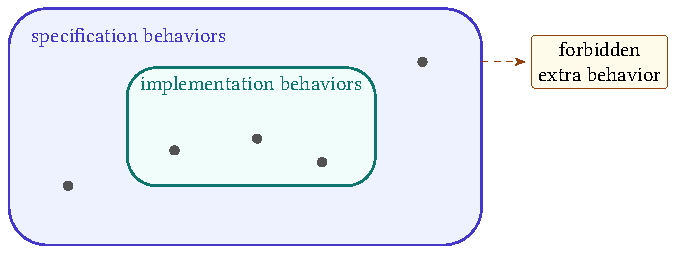
\includegraphics[width=0.88\textwidth]{figures/behavior-set-refinement}
\caption{A deterministic behavior is one path. A nondeterministic
specification admits a set; an implementation refines it when its behaviors
remain inside that set.}
\figalt{A large specification set contains several outcome points; a smaller implementation set lies inside it while one forbidden point lies outside.}
\label{fig:behavior-set-refinement}
\end{figure}

This chapter keeps the executable examples deterministic so that one trace can
explain a witness. The set view is still useful because it clarifies the
direction of refinement and prepares the boundary discussion in Chapter 16.
It also prevents an endpoint equation from being generalized beyond the model
that made it single-valued.

\section{Preconditions select the promised domain}

A \keyterm{precondition} \(\Phi(S)\) is a predicate on initial state. It can
require valid memory ranges, aligned code, nonaliasing buffers, a bounded
counter, related ABI state, or a specific operand width. Equivalence under
\(\Phi\) quantifies over every initial state satisfying it, not merely the
examples used to discover the claim.

For A0, compare these one-instruction fragments at a running aligned program
counter:

\begin{codelisting}[language={},caption={Two candidate ways to clear r0}]
P: movi r0, 0
Q: xor  r0, r0, r0
\end{codelisting}

Both leave \(r_0=0\) and advance by four on a legal fetch. They differ in
condition state: \code{movi} preserves \(Z,N,C,V\), whereas A0 \code{xor}
sets \(Z,N\) from its zero result and clears \(C,V\). Under an observation of
\(r_0\), next \(pc\), and running outcome, the fragments agree. Under full
state they generally do not.

Add the precondition that entry conditions already equal
\((Z,N,C,V)=(1,0,0,0)\). Now the two successors agree on those condition bits
as well. With unchanged remaining registers and memory, they reach the same
complete successor state. The precondition did not change either instruction;
it selected the inputs on which their complete effects coincide.

\begin{example}[title={Removing one premise produces a witness}]
Remove the entry-condition premise and choose \(C=1\). Program \(P\) preserves
\(C=1\); program \(Q\) clears it. The initial state is a concrete witness
against full-state equivalence. Appending \code{branch.hs} turns the hidden
condition difference into different control flow.
\end{example}

Preconditions must be usable by the intended caller. A theorem requiring the
two programs' outputs to be equal as an input premise is circular. A theorem
requiring a buffer range to be valid may be useful when the caller already
establishes that range. Proof systems can validate implications among
preconditions, but the book must still explain why the chosen premise matches
the application.

\begin{tryit}[title={Strengthen and weaken a claim}]
For \(P\) and \(Q\), write three contracts: result-only agreement with no
condition premise; full-state agreement with the exact condition premise; and
a false full-state claim with one premise removed. Give the witness for the
false claim before asking a solver to find it.
\end{tryit}

\subsection{Where preconditions come from}

A precondition may be inherited from a caller, derived from earlier
instructions, imposed by an ABI, or chosen to make a local optimization true.
Those sources have different proof obligations. An inherited premise must be
part of the public interface. A derived premise needs a proof from the prior
state. An ABI premise needs a pinned profile. An optimization restriction must
not exclude inputs the original program promised to handle.

For a candidate rewrite, one can ask for a \keyterm{weakest precondition}: the
largest set of initial states on which the desired agreement holds. In the
clear-register example under full-state observation, the condition tuple
must already equal the tuple written by XOR. That exact equality is the
weakest condition-state premise when all other legal-fetch premises are fixed.

Weakest does not automatically mean best. A complicated disjunction may be
hard for callers to establish or readers to understand. A slightly stronger
aligned-range premise may match a public interface better than an exact
bit-level formula. The book should state both the sufficient premise used and,
when important, whether it is known to be necessary.

\begin{example}[title={A caller must discharge the premise}]
Suppose a rewrite is valid only when carry is zero. If the preceding
instruction clears carry by its declared semantics, sequential composition can
establish the premise. If carry is merely dead after the rewrite, that does not
show it was zero before the rewrite. Entry and exit facts must not be exchanged.
\end{example}

Solver-assisted precondition discovery can suggest a condition by analyzing
counterexamples. The resulting formula remains a hypothesis until checked
against the executable semantics and simplified without changing its domain.
Discovery and theorem admission are separate routes.

\section{A hierarchy of agreement}

Let \(\Phi\) be a precondition and \(A\) an observation. For programs over the
same deterministic state space, define termination-sensitive observational
equivalence by
\[
 P\equiv_{\Phi,A}Q
 \quad\hbox{when}\quad
 \Phi(S)\Longrightarrow B_A(P,S)=B_A(Q,S)
\]
for every initial state \(S\).

Full-state equivalence is the special case in which the observation retains
the complete terminal state and behavior class. Trace equivalence is stronger
again if it requires agreement after each corresponding step. Equal final
states do not imply equal traces: one program may use a temporary register,
take more steps, or visit another control location and later restore agreement.

\begin{figure}[htbp]
\centering
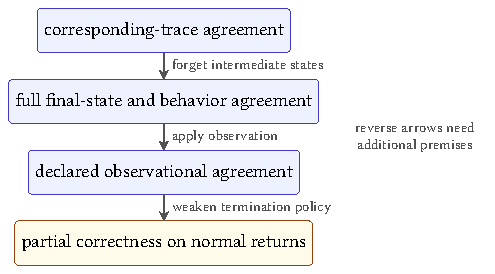
\includegraphics[width=0.82\textwidth]{figures/agreement-hierarchy}
\caption{Common agreement notions retain different information. Downward
implications hold for fixed compatible definitions; upward implications need
additional premises and usually fail.}
\figalt{Trace agreement implies full final-state agreement, which implies observational agreement, while partial correctness is weaker on termination.}
\label{fig:agreement-hierarchy}
\end{figure}

If observation \(A\) can be calculated from observation \(B\), then agreement
under \(B\) implies agreement under \(A\). The converse can fail because
\(A\) forgets information. This order lets a proof library reuse a strong
result for weaker clients without pretending that every client needs full
state.

\begin{proofkit}[title={Full-state equivalence implies observational equivalence}]
Assume both programs have the same behavior class and, on normal return, the
same complete final state for every \(S\) satisfying \(\Phi\). An observation
is a function. Applying the same function \(A\) to equal final states yields
equal results. Trap and divergence agreement is retained by the outer behavior
comparison. Therefore \(P\equiv_{\Phi,A}Q\) for every declared \(A\).
\end{proofkit}

The converse fails whenever \(A\) is not injective over reachable final
states. The clear-register example supplies two unequal condition states that
map to the same result observation. No philosophical argument is needed; the
two states and projection are enough.

\subsection{Observations form a design space}

An observation is not limited to selecting fields. It can calculate a
mathematical reading, normalize several machine outcomes, record an address
trace, or combine smaller observations. If \(A_1\) observes the result and
\(A_2\) observes memory, their product
\[
  (A_1\mathbin{\mathsf{x}}A_2)(S)=(A_1(S),A_2(S))
\]
retains both. Agreement under the product implies agreement under either
projection.

One observation is \keyterm{finer} than another when the coarser observation
can be calculated from it. Full state is finer than a register projection.
A complete trace is finer than its final state. Trap class plus reason is finer
than trap class alone. This ordering is about retained distinctions, not about
which theorem is more valuable.

The coarsest useful observation depends on the client. For a closed arithmetic
expression, one result word may suffice. For a procedure, continuation and
frame state matter. For constant-time code, an address or branch trace may
matter even when results agree. Choosing too fine an observation rejects safe
optimizations; choosing too coarse an observation accepts unsafe ones.

\begin{table}[htbp]
\centering
\caption{Sample observations and distinctions they retain.}
\begin{tabular}{@{}p{0.27\textwidth}p{0.31\textwidth}p{0.31\textwidth}@{}}
\toprule
Observation & Retains & Forgets \\
\midrule
Result word & one declared output & scratch, memory, conditions \\
Procedure result & result, outcome, continuation, frame & caller-saved scratch \\
Complete final state & every terminal component & intermediate movement \\
Address trace & selected memory locations and order & data values unless added \\
Complete trace & every selected architectural state & omitted microarchitecture \\
\bottomrule
\end{tabular}
\end{table}

Observation conversion should be explicit in a proof library. If a theorem
uses complete final state and a client needs only a result, apply the result
projection as a lemma. Do not copy the theorem and silently give its scope a
different name.

\section{Refinement relates different state spaces}

Equivalence starts both programs from one state. \keyterm{refinement} uses an
input relation \(R_{in}(S,T)\) between source state \(S\) and implementation
state \(T\), plus an output relation \(R_{out}\) between their behaviors or
terminal states. One useful deterministic form is
\[
  R_{in}(S,T)\Longrightarrow
  R_{out}(\mathit{Beh}(P,S),\mathit{Beh}(Q,T)).
\]

The relation may map A0 \(r_0\) to RV64I \code{a0}, ignore an x86-64 scratch
register, relate little-endian memory regions at different base addresses, and
connect different program-counter locations by control points. It does not
make the state spaces identical.

Refinement is directional. An implementation may allow fewer behaviors than
an abstract specification while satisfying every abstract requirement. For
our deterministic scalar slices, direction often appears only in the chosen
input and output relations. It becomes essential with \keyterm{nondeterminism},
where one input can permit several behaviors,
underspecification, concurrency, or implementation-defined choices.

\begin{keyidea}[title={A relation carries meaning across machines}]
An observation projects one state into visible information. A state relation
states when two differently shaped states represent the same abstract
situation. Cross-ISA refinement needs the relation before execution and after
execution; observation alone cannot align the machines.
\end{keyidea}

Chapter 12 develops stepwise simulations. For now, notice that endpoint
refinement can be true even when instruction counts differ. A0 may require a
comparison followed by a branch, RV64I may compare registers in the branch,
and x86-64 may read flags set earlier. The relation needs to hold at selected
entry and exit points, not after every unmatched instruction.

\section{Contexts can expose forgotten state}

A \keyterm{context} is surrounding program structure with a hole into which a
fragment is placed. Write \(C[P]\) for context \(C\) containing fragment
\(P\). A local result observation does not automatically justify
\(C[P]\equiv C[Q]\), because the suffix may read state that the local
observation forgot.

Return to \code{movi r0,0} and \code{xor r0,r0,r0}. A suffix that immediately
overwrites all conditions before reading them cannot expose their difference.
A suffix beginning with \code{branch.hs} can. Contextual replacement therefore
needs either stronger local agreement or a restriction on what the context
may observe before forgotten state is overwritten.

\begin{figure}[htbp]
\centering
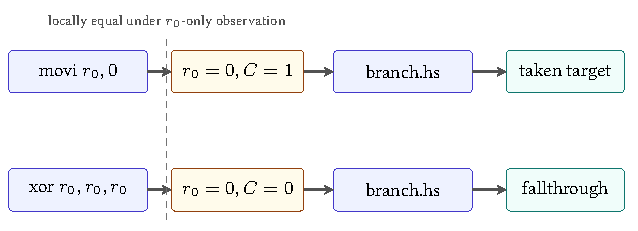
\includegraphics[width=0.9\textwidth]{figures/context-exposes-state}
\caption{A narrow local observation can hide a condition difference. A suffix
that reads carry converts it into a distinct control path.}
\figalt{Two fragments agree on r0 but leave different carry bits; appending branch.hs sends them to different successors.}
\label{fig:context-exposes-state}
\end{figure}

\begin{proofkit}[title={A sufficient contextual-replacement rule}]
Suppose fragments \(P\) and \(Q\) terminate from every allowed entry and leave
states related by \(R\). Suppose the context's next step preserves \(R\), and
every later pair of related steps preserves it until the final observation.
By induction over the context steps, the executions remain related. If
\(R\)-related terminal states have equal final observations and behavior
classes, then \(C[P]\) and \(C[Q]\) agree under that observation.
\end{proofkit}

This rule reveals the work hidden by ``the context cannot tell.'' We need a
relation after the fragment, a preservation argument for the suffix, and an
observation compatible with that relation. A read/write or liveness analysis
can establish a simpler special case when all differing locations are dead
until overwritten.

\begin{warning}[title={Dead at one point does not mean absent from the state}]
A condition bit or scratch register may be irrelevant to the current output
and live again in the next instruction. Deadness is a property of a location
relative to a program point and future uses. It is not a permanent semantic
property of the location.
\end{warning}

\subsection{Read and write sets give a practical sufficient rule}

Let \(D\) be the set of locations on which fragments \(P\) and \(Q\) may
differ at their common exit. If every path in the suffix overwrites each
location in \(D\) before reading it, and the overwrite does not itself depend
on another difference, then those exit differences cannot affect the later
observation. This is a semantic form of dead-state elimination.

The order matters. A suffix that reads carry and then overwrites all flags can
still distinguish the clear-register fragments. A suffix that first executes
an instruction with fully defined condition outputs and only then branches may
erase the difference. The proof follows paths, not just unordered read and
write sets.

Memory makes the rule relational. A store to \([p,p+8)\) overwrites a differing
byte only when the suffix's effective address is known to alias that byte. A
load through another symbolic pointer may expose it. Nonaliasing or must-alias
facts therefore become premises of the contextual proof.

\begin{proofkit}[title={Overwrite-before-read replacement rule}]
Assume \(P\) and \(Q\) terminate with states equal outside \(D\). Along every
allowed suffix path, each location in \(D\) is overwritten with equal values
before any instruction or final observation reads it. All other instructions
receive equal inputs and have deterministic equal effects. Induct over suffix
steps. After the last location in \(D\) is overwritten, the complete states
agree; the remaining execution and observation therefore agree.
\end{proofkit}

This rule is sufficient, not necessary. Two contexts may read unequal values
and nevertheless calculate equal outputs. A relational invariant can prove
that more general case. The overwrite rule is valuable because a compiler's
live-variable and effect analyses can often establish it automatically.

\section{Counterexamples should become traces}

The negation of a finite-width observational-equivalence claim asks for an
allowed initial state whose observed behaviors differ:
\[
  \Phi(S)\mathbin{\mathsf{and}}
  B_A(P,S)\ne B_A(Q,S).
\]
A solver may return assignments for thousands of internal formula variables.
Those assignments are not yet a reader-facing counterexample. Decode the
initial architectural state, run both programs through the same executable
semantics used by the claim, and print the first meaningful divergence.

\begin{figure}[htbp]
\centering
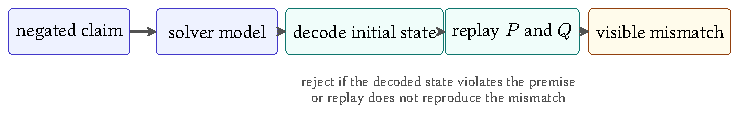
\includegraphics[width=0.92\textwidth]{figures/counterexample-replay}
\caption{A useful solver counterexample returns to the semantic level. Formula
assignments become an initial state, two checked traces, and a visible failed
observation.}
\figalt{Claim negation enters a solver; a model decodes to an initial state, replays through two programs, and yields an observation mismatch.}
\label{fig:counterexample-replay}
\end{figure}

For the clear-register pair with unconstrained carry, a compact report can
say: entry \(C=1\); \(P\) executes \code{movi} and preserves \(C=1\);
\(Q\) executes \code{xor} and writes \(C=0\); full-state comparison first
differs at carry. If a contextual claim is under test, append the branch and
show the two successor program counters as well.

The \keyterm{first divergence} depends on the comparison. Traces of unequal
length may have no step-for-step alignment. For identical one-step fragments,
the first unequal successor is clear. For optimized routines, compare related
control points or report the first violated relation rather than matching step
numbers mechanically.

\begin{example}[title={Three counterexample classes}]
An unequal final register with matching normal returns is a value witness. A
normal return on one side and a trap on the other is an outcome witness. A
pair with equal final observations but a differing intermediate secret-
dependent address is a trace witness under an address-trace observation. The
claim decides which class matters.
\end{example}

Counterexample minimization can improve explanation. Prefer small word values,
short traces, few changed memory bytes, and the earliest failing component,
provided minimization reruns the semantic checker. A smaller printed model
that no longer satisfies the formula is not evidence.

Minimization should preserve a named witness predicate. Start from a replayed
failure. Try setting irrelevant registers to zero, shrinking the initialized
memory region, simplifying word values, or lowering a loop count. After every
change, rerun the precondition, both executions, and the same observation. Keep
the change only if the same failure class remains.

The smallest numeric value is not always the clearest witness. For signed
overflow, boundary values explain the rule better than a solver's arbitrary
large assignment. For aliasing, two short visibly overlapping ranges are
better than unrelated high addresses. The minimizer can use a lexicographic
cost: behavior-class mismatch first, earliest divergence second, number of
nonzero state fields third, then magnitude.

\begin{figure}[htbp]
\centering
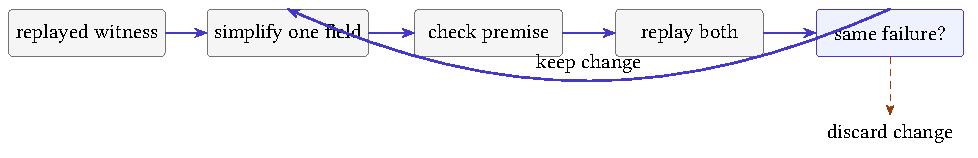
\includegraphics[width=0.86\textwidth]{figures/counterexample-minimization-loop}
\caption{Counterexample minimization is a checked loop. A proposed
simplification is kept only when semantic replay preserves the named failure.}
\figalt{A replayed witness enters simplify, precondition check, replay, and failure-class check; accepted changes loop back while rejected changes are discarded.}
\label{fig:counterexample-minimization-loop}
\end{figure}

A minimized trace should retain provenance to the original solver model. The
report records which fields changed and which checker reconfirmed the witness.
This keeps the explanatory example connected to the machine-derived result
without pretending that the minimized state was the solver's original output.

\section{Traps, undefined domains, and stuck states}

A precondition can exclude a trap only when the theorem says so. For example,
a load/store equivalence may require both byte ranges to be valid. Under that
premise, no range trap occurs. Without it, the programs may trap differently
because they compute different addresses or access different widths.

Do not confuse an undefined mathematical helper with an architectural trap.
A partial specification function may be undefined outside its domain. An A0
running step instead produces a declared trapped outcome for an invalid data
range or illegal instruction. A semantics can also become accidentally
\emph{stuck} if no rule applies and no trap was defined. Total executable
semantics should distinguish legal successor, declared trap, terminal input,
and malformed external data.

Trap equivalence itself has choices. A narrow claim may require only that both
sides trap. A stronger claim may require the same reason and preserved state.
An even stronger platform claim may expose fault addresses or exception codes.
Print which trap observation is used; ``both fail'' is not a complete rule.

\begin{tryit}[title={Choose a trap observation}]
Construct two A0 loads that both access outside finite memory but begin from
different destination-register values. Compare them under three policies:
trap class only; trap class and reason; complete trapped state. Identify which
differences each policy can expose.
\end{tryit}

\section{Composing equivalence claims}

Equivalence is reflexive, symmetric, and transitive when its precondition,
behavior policy, semantics, and observation are fixed appropriately. These
properties permit chains of validated rewrites, but changing a scope in the
middle can break the chain.

Suppose \(P\equiv_{\Phi,A}Q\) and \(Q\equiv_{\Phi,A}R\). For every allowed
state, equality of observed behavior gives \(B_A(P,S)=B_A(Q,S)\) and
\(B_A(Q,S)=B_A(R,S)\). Transitivity of equality yields
\(B_A(P,S)=B_A(R,S)\). If the first claim instead uses precondition \(\Phi_1\)
and the second \(\Phi_2\), the composed claim needs at least their conjunction
or another premise implying both.

Sequential composition also needs an intermediate-domain argument. If
fragments \(P_1\) and \(Q_1\) leave related states, and \(P_2\) and \(Q_2\)
agree only for states satisfying \(\Psi\), then the first pair must establish
\(\Psi\) for the second. Matching endpoint observations from the first pair
may be too weak to establish that premise.

\begin{goingdeeper}[title={Congruence is equivalence that survives construction}]
An equivalence relation is a congruence for a program constructor when
replacing related parts inside that constructor preserves the relation.
Contextual equivalence asks for agreement in every allowed context and is
therefore designed for replacement. Directly proving all contexts is often
hard; simulations, logical relations, type systems, and effect analyses supply
tractable sufficient conditions.
\end{goingdeeper}

\subsection{Refinement relations compose through an intermediate state}

Suppose \(P\) refines to \(Q\) through relations \(R_{in}^{PQ}\) and
\(R_{out}^{PQ}\), and \(Q\) refines to \(R\) through corresponding relations
for \(QR\). Composition needs an intermediate witness: for every related
\(P\)- and \(R\)-entry pair, there must be a \(Q\) entry satisfying both input
relations. The two output relations must likewise imply the desired direct
\(PR\) relation.

Writing this witness explicitly prevents a common gap. One proof may interpret
a buffer at base \(a\); the next may expect it at base \(b\). One may expose
normal-versus-trap outcome; the next may forget trap reason. One may require a
preserved register that the next treats as scratch. The shared program name
\(Q\) does not guarantee that its two contracts meet.

\begin{proofkit}[title={Relational composition pattern}]
Choose intermediate entry \(T\) such that
\(R_{in}^{PQ}(S,T)\) and \(R_{in}^{QR}(T,U)\). Apply the first refinement to
relate the behavior of \(P\) from \(S\) to \(Q\) from \(T\). Apply the second
to relate that same \(Q\) behavior to \(R\) from \(U\). Finally use a relation-
composition lemma showing that the two output relations imply
\(R_{out}^{PR}\). Quantify over every direct input pair for which such a
compatible \(T\) is guaranteed.
\end{proofkit}

In a compiler pipeline, the intermediate witness is often a translated program
plus related state. In a cross-ISA proof, it may be an A0 state that both real
machines represent. In an optimization chain, it may simply be the common
machine state. The pattern is the same; only the relations change.

Optimization pipelines should record the exact contract of each rewrite.
Combining destination-only, flag-sensitive, memory-sensitive, and
termination-insensitive facts without conversion lemmas can produce an
unsupported final claim even when every individual checker returns success.

\section{Four ways to check a finite equivalence claim}

Direct testing runs selected examples. It is fast and excellent for debugging,
but its conclusion covers only those examples. Exhaustive enumeration covers
every state in a genuinely finite declared domain; it becomes expensive as
width, registers, memory, or program length grows.

Symbolic execution represents many inputs with expressions and accumulates
path conditions. It can expose how a disagreement depends on an input and can
feed a solver. A direct solver encoding instead asks whether the precondition
and observation mismatch are jointly satisfiable. Both routes rely on the
sound connection between machine semantics and generated formulas.

A reader proof can establish a parametric law, such as XOR clearing a register
at every width, when the definitions admit algebraic reasoning. A proof
assistant can check that argument against formal definitions. These methods
are complementary: tests diagnose, enumeration calibrates tiny domains,
solvers search wide finite spaces, and proofs explain universal structure.

\begin{table}[htbp]
\centering
\caption{Checking routes support different scopes.}
\begin{tabular}{@{}p{0.22\textwidth}p{0.31\textwidth}p{0.36\textwidth}@{}}
\toprule
Route & Strongest direct scope & Central risk \\
\midrule
Examples & named initial states & untested inputs \\
Enumeration & complete finite declared domain & omitted states or transitions \\
Solver query & generated finite formula & encoding and verdict trust \\
Formal proof & stated theorem over formal definitions & definition and assumption boundary \\
\bottomrule
\end{tabular}
\end{table}

Agreement among routes is valuable but does not merge their scopes. If a
direct-enumeration tool and solver agree at width eight, that cross-checks two
implementations on one finite domain. A width-parametric proof needs its own
argument. Conversely, a proof over an abstract step rule does not validate a
decoder until bytes are connected to that rule.

The practical sequence mirrors the book's pedagogy. Start with a hand-chosen
witness and its complete trace. Enumerate a miniature width to test the state
inventory. Generalize the disagreement formula and ask a solver for a model.
Replay every returned model. Only then invest in a certificate or parametric
proof whose exact statement has survived those cheaper attacks. Each stage
sharpens the claim carried by the next.

\section{An introductory Axeyum equivalence route}

The current Axeyum checkout supplies bit-vector and solver infrastructure but
does not yet contain the executable A0 program layer required by this chapter.
The first sound route begins only after \code{a0-state}, \code{a0-step}, and
\code{a0-run} exist with their negative controls.

Represent an equivalence query with semantic-package digests, two decoded
programs, word width, precondition, behavior policy, observation, and a bound
or termination argument. Generate the negation of the exact reader statement.
For a satisfiable result, decode the model into a complete A0 initial state and
replay both programs. Reject the evidence if replay does not reproduce the
claimed mismatch.

For an unsatisfiable result, preserve the formula and solver configuration.
The strongest available route should export independently checkable evidence
or reconstruct the theorem in a kernel. The assurance label must still say
whether the result covers one width, a finite width set, or a width-parametric
statement.

\begin{example}[title={The first A0 equivalence query}]
Compare \code{movi r0,0} with \code{xor r0,r0,r0}. Query result-only
equivalence first; a deliberate destination mutation must produce a replayed
witness. Then query full-state equivalence without the condition premise; the
tool should find a condition-state witness. Finally add the exact premise and
check the stronger claim. The sequence tests both proof and counterexample
paths without requiring a long program.
\end{example}

Negative controls must target every layer. Mutate a destination or condition
effect in A0 semantics. Omit one observed component. Invert the precondition.
Corrupt one decoded model field before replay. Change the formula digest after
the solver runs. A route that rejects only false programs but accepts a stale
formula or nonreplaying model has not established the advertised claim.

\begin{proofkit}[title={Why replay is load-bearing}]
The solver establishes a result about the generated formula. Replay checks
that a satisfying assignment decodes to an allowed architectural state and
that executable semantics produces the reported difference. Without replay,
a bug in formula generation or model decoding can manufacture a persuasive
but irrelevant assignment. Replay does not validate an unsatisfiable verdict;
that needs formula provenance and a certificate or stronger checking route.
\end{proofkit}

The Python or PyO3 surface should make the teaching path small: construct two
programs, choose a named observation, state a precondition, request a check,
and receive either bounded evidence or a typed counterexample trace. The lower
Rust layer owns semantic definitions, digests, solver translation, and replay.
The convenient interface must not invent a broader result than the evidence
returned by that layer.

\section{Where the equivalence model stops}

This chapter uses deterministic sequential architectural behavior. It does not
cover concurrency, weak memory, probabilistic behavior, external input during
execution, interactive systems, fairness, timing, energy, cache traces,
speculation, or quantitative leakage. Each can require sets or distributions
of behaviors and richer observations.

It also introduces refinement without yet proving a cross-ISA simulation.
Chapter 12 supplies control-point relations, stuttering, and forward-simulation
reasoning. Chapter 13 adds program languages and costs; agreement alone says
nothing about minimality or speed.

Within the boundary, a precise equivalence statement turns optimization from
hope into a refutable claim. The counterexample is not an embarrassment. It is
the smallest state in which our promised sameness breaks, and therefore one of
the clearest explanations the machine can give us.
Preserving that explanation requires the report to retain the starting state,
both outcomes, the selected observation, and the first component that violates
the relation. A bare Boolean loses the lesson at the moment it finds the bug.

\section{Exercises}

\begin{enumerate}
\item Give two A0 final states related by an \(r_0\)-only observation but
separated by a full-register observation, a condition observation, and an
outcome observation.

\item \textbf{Execute.} Trace \code{movi r0,0} and
\code{xor r0,r0,r0} from entry conditions \((0,1,1,1)\). List the complete
successors and their first differing components.

\item State the weakest observation in which the two clear-register fragments
agree without a condition precondition. Explain one context that makes that
observation insufficient for replacement.

\item \textbf{Prove.} Prove their full-state equivalence under the exact entry-
condition premise printed in this chapter. Include unchanged registers,
memory, program counter, and outcome.

\item \textbf{Break.} Remove each condition conjunct from that premise in
turn. Give a concrete entry state when removal makes the full-state claim
false, or explain why a conjunct was redundant.

\item Give a pair of programs with equal final states but different trace
lengths. State a final-state observation that equates them and a trace
observation that separates them.

\item Distinguish normal return, trap, divergence, and bound exhaustion. Which
are architectural behaviors in the model, and which is a runner result?

\item Write a partial-correctness statement that permits termination mismatch.
Explain why it cannot alone authorize replacement in a terminating context.

\item Let observation \(A\) be computable from \(B\). Prove that agreement
under \(B\) implies agreement under \(A\). Give a noninjective counterexample
to the converse.

\item Define input and output relations between the A0, RV64I, and x86-64 add-
one procedures from Chapter 10. Do not require identical register names or
program-counter values.

\item \textbf{Transfer.} State endpoint refinement for those three procedures,
including behavior class, result, continuation, stack restoration, preserved
state, and memory.

\item Build a suffix that observes the carry difference between the two A0
clear-register fragments. Trace the first control-flow divergence.

\item Prove the sufficient contextual-replacement rule for a suffix of \(n\)
steps by induction on \(n\).

\item Give two trapping A0 executions that agree under trap-class observation
but differ under a complete trapped-state observation.

\item Show how preconditions compose when \(P\equiv_{\Phi_1,A}Q\) and
\(Q\equiv_{\Phi_2,A}R\). State a sufficient premise for relating \(P\) and
\(R\).

\item Design a counterexample report containing initial state, semantic
digests, both traces, first violated relation, and final observations. Explain
which fields a reader needs and which solver-internal fields may remain
archived.

\item Design the first Axeyum A0 equivalence manifest. Include the exact query,
width, precondition, observation, behavior policy, expected result, replay
command, formula digest, and five negative controls.

\item A solver returns a model that fails executable replay. Give at least
three possible fault classes and explain why the original equivalence verdict
cannot use that model as evidence.
\end{enumerate}
